% \section[toc={JOS Courses}]{JOS Courses}

% Assumes in caller: \usepackage{etoolbox} % for \newtoggle et al
\newtoggle{pmyear}
\togglefalse{pmyear}

%\begin{wideslide}[\slideopts]{JOS Courses After Music 320 A and B}
%\begin{wideslide}[\slideopts,toc={JOS Courses}]{JOS Research Courses}
\begin{slide}[\slideopts,toc={Courses}]{Courses Developed for CCRMA}
%\vspace{-1em}

%\myTwoFiguresToWidth{icon-57}{outer_ear}{0.1\twidth}{MUS420}{MUS421}{}

% FIXME: These need to be listed as Marina or JOS 320E:
\newcommand{\mdftcourse}{\htmladdnormallink{\textbf{Music 320A}}{https://ccrma.stanford.edu/courses/320/}: \textsc{Audio Spectrum Analysis}}
\newcommand{\josfpcourse}{\htmladdnormallink{\textbf{Music 320B}}{https://ccrma.stanford.edu/courses/320/}: \textsc{Audio Filter Analysis and Structures}}
\newcommand{\paspcourse}{\htmladdnormallink{\textbf{Music 420A}}{https://ccrma.stanford.edu/courses/420/}: \textsc{\textbf{\large Physical} Audio Signal Processing}}
\newcommand{\saspcourse}{\htmladdnormallink{\textbf{Music 421A}}{https://ccrma.stanford.edu/courses/421/}: \textsc{\textbf{\large Time-Frequency} Audio Signal Processing}}

\begin{itemize}
\mpitem \mdftcourse
\item[]
\mpitem \josfpcourse
\item[]
\mpitem \iftoggle{pmyear}{\saspcourse}{\paspcourse}
\item[]
\mpitem \iftoggle{pmyear}{\paspcourse}{\saspcourse}
\end{itemize}

\maybepause

\vspace{-1em}
\begin{center}
\vcenteredhbox{\resizebox{0.2\textwidth}{!}{\includegraphics{eps/icon-57.eps}}}
\qquad 
% 420 
\quad $\mathbf{\longrightarrow}$ \quad 
% 421
\qquad\;
\vcenteredhbox{\resizebox{0.2\textwidth}{!}{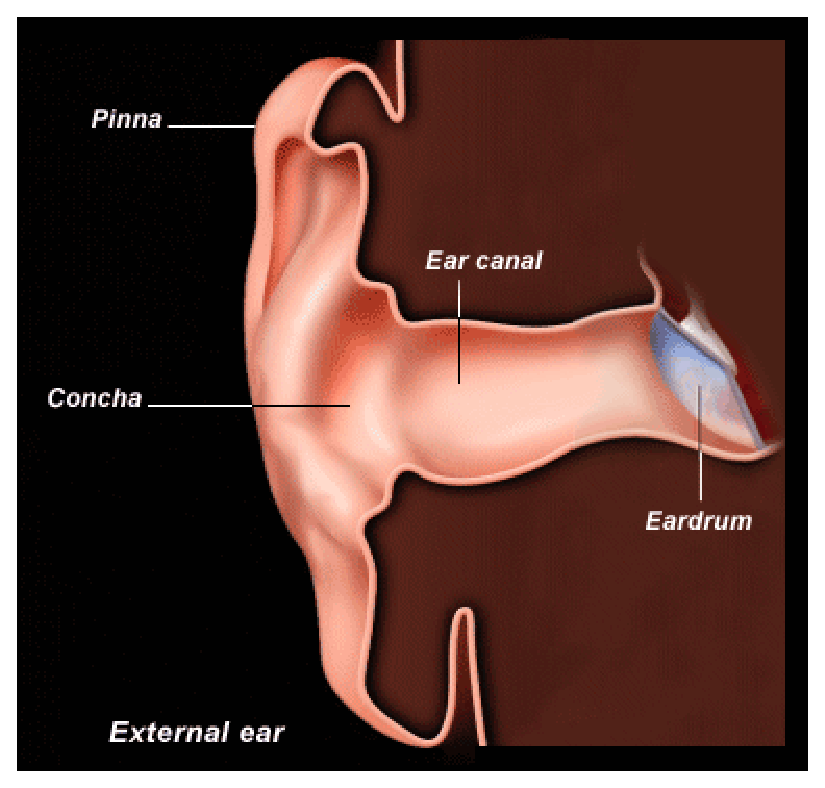
\includegraphics{eps/outer_ear.eps}}}\\
\makebox[0.2\textwidth][c]{420A}
\qquad 
% 420 
\quad\!\!
\qquad\quad % ~ width of $\mathbf{\longrightarrow}$
\quad 
% 421
\qquad
\makebox[0.2\textwidth][c]{421A}
\end{center}
\vspace{-1em}

%\item \textbf{Music 421B} (Spr): 421 Projects in SuperCollider, C++, and/or Matlab
%\item \textbf{Music 420B} (Spr): 420 Projects in Faust, C++, and/or Matlab
%\resizebox{0.1\twidth}{!}{\includegraphics{eps/icon-57.eps}}
%\myFigureToWidth{icon-57}{0.3\twidth}{}
%\myFigureToWidth{outer_ear}{0.3\twidth}{}
%\resizebox{0.1\twidth}{!}{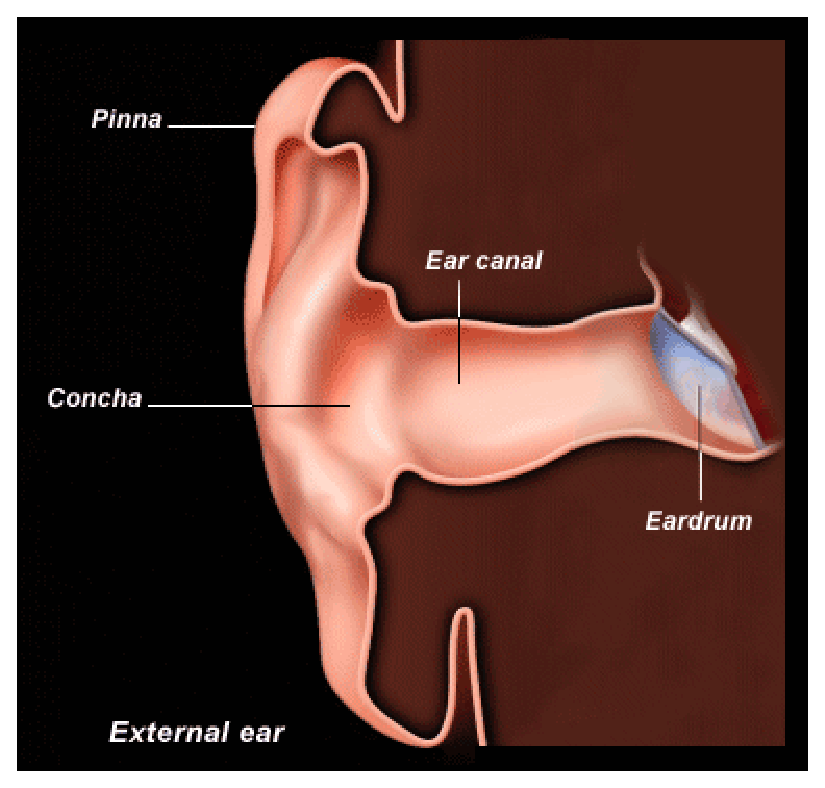
\includegraphics{eps/outer_ear.eps}}
%\myTwoFiguresToBoxes{icon-57}{outer_ear}{0.4\twidth}{0.6\textheight}{Source}{Listener}{}

\maybepause

\centerline{All four textbooks \htmladdnormallink{\textbf{free online}}{http://ccrma.stanford.edu/~jos/\#books}}

\end{slide}

%% \begin{slide}[\slideopts,toc={JOS Seminars}]{JOS Research Seminars}
%% \BIT
%% \item \textbf{Music 322 (Fall):}\\ \textsc{Music/Audio Signal Processing Research Overviews}
%% \vspace{1em}
%% \item \textbf{Music 423 (All Quarters):}\\ \textsc{Music/Audio Signal Processing Research}
%% \EIT
%% \end{slide}
